\documentclass[conference]{IEEEtran}
\IEEEoverridecommandlockouts
\usepackage{cite}
\usepackage{amsmath,amssymb,amsfonts}
\usepackage{graphicx}
\usepackage{booktabs}
\usepackage{multirow}
\usepackage{xcolor}
\usepackage{url}
\graphicspath{{figures/}}
\newcommand{\pmsd}[2]{#1{\scriptsize$\pm$#2}}
\newcommand{\ci}[3]{#1{\scriptsize\,[#2,\,#3]}}

\begin{document}

\title{Screening for Dyslexia, Dyscalculia and Dysgraphia from One Tablet Session:\\
A Realistic Synthetic Benchmark, an Age- and Language-Normed Pipeline,\\
and Lessons from a Deployment Audit}

\author{
\IEEEauthorblockN{[Author Name]\IEEEauthorrefmark{1}, [Co-author Name]\IEEEauthorrefmark{1}, [Supervisor Name]\IEEEauthorrefmark{2}}
\IEEEauthorblockA{\IEEEauthorrefmark{1}[Department], [Institution], [City, Country]}
\IEEEauthorblockA{\IEEEauthorrefmark{2}[Department], [Institution], [City, Country]\\
Email: [corresponding author e-mail]}
}

\maketitle

\begin{abstract}
Specific learning disorders in reading, mathematics and written expression often
co-occur and are under-identified where specialists are scarce. We study SwarSetu, a
tablet screen that scores all three disorders from one session of reading, arithmetic
and handwriting tasks. Its published synthetic benchmark was too easy: plain logistic
regression reached AUROC 0.96 because the per-feature effect size was $d\approx1.5$,
not the stated 0.6. We replace it with a liability-threshold cohort generator that
models correlated abilities, comorbidity, age and home-language confounds, device
effects, missing data and imperfect diagnoses. On five seeds ($n{=}6000$) plus a
shifted external site, the proposed FT-Transformer reaches macro AUROC 0.804, no
better than logistic regression (0.807). A LightGBM pipeline on age- and
language-normed features reaches 0.858 (95\% CI 0.846--0.869), beats every other
model by $\geq$0.007 AUROC in paired bootstrap tests, is calibrated (ECE 0.017),
gives class-conditional conformal coverage of 0.94/0.90, and narrows subgroup gaps
in false positives. It is best or within 0.005 of best in all 22 settings of a
generator sensitivity analysis. The advantage comes mainly from handling the age
confound: without it, all models converge. For handwriting, the original scorer
measured the input device rather than the child: neat writing scored 54--62/100
on touch and mouse. A device-invariant analysis with a self-hosted handwriting
recogniser scores neat synthetic writing 99--100 on every device and flags 11 of
12 impaired writers. Speech input now uses a self-hosted Whisper model. An audit
found 17 defects that together made the deployed screen flag no child. We then align
the screen with DSM-5: a teacher questionnaire records Criteria A--D, each test reports
the DSM-5 specifiers (adding oral reading fluency, timed number facts and dictation,
sentence and composition tasks), and a domain-specific Criterion D rule routes
children whose difficulties may reflect language, vision or hearing to review. The
questionnaire adds no significant discrimination ($+0.001$ AUROC, 95\% CI $-0.002$ to
$0.004$); its value lies in the criteria the tests cannot observe. All results are
synthetic and do not estimate clinical accuracy.
\end{abstract}

\begin{IEEEkeywords}
dyslexia, dyscalculia, dysgraphia, early screening, synthetic data, gradient boosting,
calibration, conformal prediction, fairness, handwriting analysis, ML system audit
\end{IEEEkeywords}

%=====================================================================
\section{Introduction}
%=====================================================================
DSM-5 groups impairments in reading (dyslexia), mathematics (dyscalculia) and written
expression (dysgraphia) under one diagnosis of specific learning disorder, with a
school-age prevalence of 5--15\%~\cite{dsm5}. A quarter to a half of children with one
of these disorders also meet the criteria for another~\cite{willcutt2013,landerl2010},
as multiple-deficit models predict~\cite{pennington2006}. Intervention works best in
the primary grades, but formal assessment needs specialists who are scarce in many
school systems. A short, cheap screen that a teacher can run, covering all three
disorders, could help decide who needs a specialist.

SwarSetu is such a screen. Children complete reading, arithmetic and handwriting
tasks on a tablet; a model scores the risk of each disorder. Its earlier evaluation
reported an AUROC near 0.97 on synthetic data. Before a tool like this reaches
children, we need to know whether that evaluation reflects real measurement
conditions, which model to use, and whether the deployed software computes what was
evaluated. This paper makes six contributions:
\begin{enumerate}
\item A \emph{realistic synthetic cohort generator} for joint screening of the three
disorders (Section~\ref{sec:cohort}). Comorbidity, confounding and measurement
artefacts arise from a liability-threshold model rather than being imposed on labels.
\item A \emph{screening pipeline} that norms features for age and home language, uses
gradient boosting, pre-registered operating points and class-conditional conformal
sets, and stores model, preprocessing and thresholds in one verified bundle
(Section~\ref{sec:pipeline}).
\item An \emph{evaluation} of 15 model variants over five seeds and an external site,
with paired bootstrap intervals, learning curves and a 22-setting sensitivity
analysis of the generator's assumptions (Sections~\ref{sec:protocol}--\ref{sec:results}).
\item A \emph{device-invariant handwriting analysis} with self-hosted legibility
recognition, and self-hosted speech recognition (Section~\ref{sec:handwriting}).
\item A \emph{DSM-5 alignment}: a stored student profile and teacher questionnaire for
Criteria A--D, specifier-level subtests, and an evaluation of what the questionnaire
and a Criterion D exclusion rule add (Sections~\ref{sec:dsm5} and~\ref{sec:dsm5res}).
\item A \emph{deployment audit} with executable checks, reported as lessons
(Section~\ref{sec:audit}).
\end{enumerate}
All data are synthetic. The results test the pipeline under plausible conditions;
they do not estimate clinical accuracy (Section~\ref{sec:limits}).

%=====================================================================
\section{Related Work}
%=====================================================================
Machine-learning screens have mostly targeted one disorder: eye-tracking during
reading for dyslexia~\cite{rello2015} and tablet handwriting kinematics for
dysgraphia~\cite{asselborn2018}. On tabular data of moderate size, gradient-boosted
trees usually match or beat deep networks~\cite{grinsztajn2022}, including
FT-Transformers~\cite{gorishniy2021}. Calibration matters when probabilities drive
referrals~\cite{guo2017}, and split conformal prediction gives distribution-free
coverage~\cite{angelopoulos2021}; class-conditional (Mondrian)
variants~\cite{vovk2005} give that guarantee to each class separately, which matters
when the class of interest is rare. Group fairness at a fixed operating point can be
assessed through equal opportunity~\cite{hardt2016}. Production ML systems often
fail through pipeline problems such as train/serve skew rather than through the
model itself~\cite{sculley2015}. We follow the reporting spirit of
TRIPOD~\cite{collins2015}.

%=====================================================================
\section{System}
%=====================================================================
\subsection{Tasks and features}
Four extractors map task telemetry to 16 features each, scaled to $[0,1]$ with higher
values meaning better performance:
(i)~reading: speed relative to an age norm, accuracy, phoneme errors, letter
confusions, pseudoword decoding, rapid automatised naming, phonological awareness,
comprehension;
(ii)~mathematics: subitising, comparison speed, fact retrieval, number line, place
value, multi-step accuracy, word problems;
(iii)~handwriting: speed, pressure, straightness, smoothness, tremor, alignment, size
consistency, pauses, pen lifts, baseline drift and composites;
(iv)~behaviour: attention, persistence, impulse control and related executive
measures. Missing inputs receive fixed defaults (0.5 or 0.7). Only reading speed is
age-normed by the extractors.

\subsection{Originally proposed model}
The original model is an FT-Transformer-style network~\cite{gorishniy2021} (1.06\,M
parameters): four 16-feature domain tokens, self-attention, residual MLP blocks and
a learnable label-correlation layer. It is trained with an asymmetric loss
(ASL)~\cite{benbaruch2021} plus a Dice term, uses 30 Monte-Carlo dropout
passes~\cite{gal2016} and temperature scaling~\cite{guo2017} at inference, and
thresholds each disorder with a weighted Youden index~\cite{youden1950}. For a single
test, the other 48 features are filled with 0.5.

%=====================================================================
\section{Realistic Synthetic Cohorts}\label{sec:cohort}
%=====================================================================
\subsection{Why the original benchmark is too easy}
The original generator lowers all 16 features of a disorder's block by a constant and
then min--max normalises the full dataset. The stated effect size of 0.6 is applied
in units whose noise SD is 0.3, so the median per-feature Cohen's $d$ is 1.50--1.63
and prevalence is 16--21\% instead of 15\%. Logistic regression alone reaches test
AUROCs of 0.96--0.97, so the benchmark cannot separate models.

\subsection{Generative model}
Each child has five correlated latent abilities: reading/phonology $R$, number sense
$M$, graphomotor control $W$, executive attention $E$ and processing speed $S$
($\rho_{RM}{=}0.55$, $\rho_{RW}{=}0.40$, others 0.25--0.40). Disorder $k$ is present
when its liability falls below the prevalence quantile~\cite{falconer1965}:
\begin{equation}
\ell_k = r\,\tilde z_k + \sqrt{1-r^2}\,\varepsilon_k,\qquad y_k=\mathbb{1}[\ell_k<\Phi^{-1}(\pi_k)],
\end{equation}
where $\tilde z_k$ is the standardised primary latent ($R$, $M$, or $0.85W{+}0.25R$),
$r{=}0.9$ is diagnostic reliability and $\pi{=}(0.08,0.06,0.07)$. Comorbidity arises
from the latent correlations: $P(\text{DCL}\mid\text{DLX}){=}0.22$,
$P(\text{DLX}\mid\text{DCL}){=}0.29$, $P(\text{DLX}\mid\text{DGR}){=}0.30$, within
published ranges~\cite{willcutt2013,landerl2010}.

The 64 features keep the semantics, polarity, defaults and derived formulas of the
production extractors. Each is a noisy combination of one or more latents (loadings
0.15--0.75), including deliberate cross-domain loadings (word problems load on $M$
and $R$). Median per-feature effect sizes are $d{=}0.77$, 0.91 and 0.81, close to
meta-analytic estimates~\cite{melbylervag2012}. The generator adds:
\begin{itemize}
\item \emph{development}: raw skills rise by 0.25\,SD per year from age 7 to 13;
\item \emph{home language}: 60\% of children are Hindi-dominant and score 0.35\,SD
lower on English phonological and comprehension items without a disorder;
\item \emph{input device}: 70\% use a finger, so pressure is unavailable and
kinematics are noisier;
\item \emph{secondary effects}: lower frustration tolerance and persistence with any
disorder;
\item \emph{measurement}: binomial item scores (7--30 items), a reading-speed ceiling
hit by 38\% of children, 8\% missing items and 10\% skipped modules filled with the
extractor defaults;
\item \emph{reference standard}: 10\% of true cases are labelled negative and 1\% of
typical children positive.
\end{itemize}
An external site (Site~B) shifts every factor: younger children, 85\% Hindi-dominant,
95\% finger input, extra noise, more missing data and 25\% higher prevalence. Because
of label noise, an oracle knowing each child's true latent driver reaches AUROC
0.89--0.91, and logistic regression trained on 30{,}000 children reaches 0.84--0.85.

%=====================================================================
\section{Screening Pipeline}\label{sec:pipeline}
%=====================================================================
\textbf{Norming.} Psychometric tests are scored against age norms. We do the same
statistically: on typically-developing training children, each feature $x_j$ is
regressed on covariates $c=(a,a^2,h,f)$ (age, age squared, Hindi-dominant, finger
input), and the model receives the standardised residual
\begin{equation}
z_j = \bigl(x_j - \hat\beta_j^{\top} c\bigr)/\hat\sigma_j .
\end{equation}
Unknown covariates are imputed with training means; 15\% of training covariates are
masked so that the model is trained for that case.

\textbf{Model.} The normed features plus 64 missing-input indicators feed one
LightGBM classifier~\cite{ke2017} per disorder (300 trees, 7 leaves, learning rate
0.03). A \emph{comprehensive} model uses all 64 features; three \emph{single-test}
models use only their 16-feature block, replacing the 0.5-fill strategy.

\textbf{Operating points and uncertainty.} On held-out validation data we set a
\emph{refer} threshold at sensitivity $\geq$0.85 and a \emph{monitor} threshold at
$\geq$0.95, giving three reachable tiers. For each class we compute split-conformal
quantiles of the score $1-\hat p(\text{true class})$ separately
(Mondrian~\cite{vovk2005}, $\alpha{=}0.1$). The prediction set
($\{0\}$, $\{1\}$ or $\{0,1\}$) is reported as screen-negative, screen-positive or
\emph{uncertain} (re-screen). TreeSHAP~\cite{lundberg2020} values give the main
skills behind each result.

\textbf{Packaging.} Normer, models, thresholds and conformal quantiles are saved in a
single JSON bundle with a SHA-256 checksum, verified against the extractors' feature
names at load. Every screening input, feature vector, prediction and model version is
stored in PostgreSQL, together with any later confirmed diagnosis, so that real
labelled data accumulate for re-training.

%=====================================================================
\section{Handwriting and Speech}\label{sec:handwriting}
%=====================================================================
\subsection{A device-invariant dysgraphia analysis}
The original scorer computed smoothness, tremor and precision on raw pointer
samples. Touch and pen screens report 120--240 events per second, so samples are
1--2\,px apart and pixel quantisation looks like tremor; its ``precision''
(chord/path) also penalised every curved letter. We replace it with four domains
computed per drawing:

\emph{Motor control.} Each stroke is resampled to 1\,px, lightly smoothed to remove
quantisation, and resampled at 3\% of the stroke's own size. With $L_\sigma$ the
path length after Gaussian smoothing of width $\sigma$ samples, the jitter index is
\begin{equation}
J = L_{1}/L_{4} - 1 ,
\end{equation}
the extra length that high-frequency oscillation adds. Because it is measured relative
to each stroke's size, it does not depend on sampling rate, screen size or letter size.

\emph{Fluency.} Speed in letter-heights per second, mid-stroke halts (smoothed speed
below 15\% of the stroke median for $\geq$120\,ms) and pauses between strokes, with
expectations set per device type. Mouse input is flagged as unreliable for fluency
and down-weighted.

\emph{Layout.} For words, the robust slope of letter bottoms and the scatter of letter
bottoms and tops, ignoring dots, crossbars and descenders.

\emph{Legibility.} A self-hosted handwriting recogniser, TrOCR~\cite{li2023trocr},
reads each letter or word; legibility is $1-\text{CER}$ against the prompt. Simple
shapes are checked geometrically (closure, roundness, corner count). Devanagari text
and free drawings are reported as not assessed.

Scores are combined with weights 0.40 (legibility), 0.25 (fluency), 0.20 (motor) and
0.15 (layout). A domain below 60 makes the result at least moderate risk.

\subsection{Speech}
Spoken answers in the reading, working-memory and perception tasks are transcribed
by a self-hosted Whisper model~\cite{radford2023whisper} (large-v3-turbo on GPU,
small on CPU). Audio is segmented at pauses in the browser and each segment is
transcribed once. Silent clips return an empty transcript instead of a hallucinated
one. Oral reading fluency is scored by aligning the transcript with the passage
(Section~\ref{sec:dsm5}).

%=====================================================================
\section{DSM-5 Alignment}\label{sec:dsm5}
%=====================================================================
DSM-5 diagnoses a specific learning disorder when (A)~at least one of six symptoms has
persisted for six months despite targeted help, (B)~attainment is well below that
expected for age and interferes with schooling, (C)~difficulties began in the school
years, and (D)~they are not better explained by intellectual disability, uncorrected
vision or hearing problems, other mental or neurological disorders, psychosocial
adversity, lack of proficiency in the language of instruction or inadequate
instruction~\cite{dsm5}. Tests can only speak to Criterion~B. A screen that ignores A,
C and D will refer children whose difficulty has another cause.

\subsection{Student profile and teacher questionnaire}
After a teacher adds a child and grade, the teacher or an operator completes a
profile (Table~\ref{tab:questionnaire}): date of birth, home language, language of
instruction, input device, and items for each criterion. Answers are validated against
a schema served by the backend, stored per student with full history, and reused at
every assessment: age, home language and device feed the model's covariates, so they
are no longer imputed. Six questionnaire features (symptom frequency and teacher-rated
attainment for reading, writing and mathematics) enter the model as optional inputs;
when absent they are passed as missing values, which LightGBM handles natively.

\begin{table}[!t]
\centering
\caption{Teacher/operator questionnaire, by DSM-5 criterion.}
\label{tab:questionnaire}
\footnotesize
\setlength{\tabcolsep}{3pt}
\begin{tabular}{@{}lp{6.6cm}@{}}
\toprule
Part & Items \\
\midrule
Details & Date of birth (age), gender, home and instruction language, input device, handedness, years in school, attendance \\
A & Frequency (never--very often) of the six symptoms: word reading, comprehension, spelling, written expression, number sense/facts, math reasoning; duration $\geq$6 months; targeted help received and response \\
B & Attainment in reading, writing and mathematics relative to the class; interference with school work \\
C & Onset during the school years \\
D & Vision, hearing, proficiency in the language of instruction, interrupted schooling, suspected intellectual disability, neurological condition, psychosocial adversity, attention \\
History & Speech delay, family history, prior assessment, notes \\
\bottomrule
\end{tabular}
\end{table}

\subsection{Specifier-level subtests}
Each test now reports the DSM-5 specifiers of its domain (Table~\ref{tab:specifiers}).
Three subtests were added because the original tasks did not measure a specifier.
\emph{Oral reading fluency}: the child reads a graded passage aloud for up to a
minute; the Whisper transcript is aligned with the passage by a semi-global edit
distance that lets the child stop anywhere, does not count repetitions as words read,
and tolerates a one-letter recognition slip on words of five letters or more. Words
correct per minute (WCPM) are compared with published English norms~\cite{hasbrouck2017};
a teacher-scored mode (tap misread words) covers classrooms without a microphone.
Before this change the reading rate sent to the model was a constant multiple of the
number of questions answered. \emph{Number facts}: one minute of grade-appropriate
facts on an on-screen keypad gives facts correct per minute, accuracy and time per
correct fact (retrieval speed). \emph{Written expression}: the dysgraphia task now
separates copying (letters and one word, for legibility and pen control) from
dictation (words spoken by text-to-speech and not shown, for spelling), a dictated
sentence (capitalisation, punctuation, omissions) and, from Grade~3, a two-sentence
composition. The handwriting recogniser pre-marks spelling; the teacher confirms each
item and rates the composition's clarity and grammar on a three-point scale.
Handwriting measures are kept as supporting evidence: when handwriting is weak but
spelling, grammar and clarity are not, the report points to developmental
coordination disorder (an occupational-therapy check) rather than an SLD.

\begin{table}[!t]
\centering
\caption{DSM-5 specifiers and the tasks that measure them. New tasks in bold.}
\label{tab:specifiers}
\footnotesize
\setlength{\tabcolsep}{3pt}
\begin{tabular}{@{}lp{2.6cm}p{4.0cm}@{}}
\toprule
Domain & Specifier & Task and measure \\
\midrule
\multirow{3}{*}{Reading} & Word reading accuracy & Phonological awareness, pseudowords; \textbf{passage word accuracy} \\
 & Reading rate or fluency & \textbf{Oral reading: WCPM} \\
 & Comprehension & Passage questions \\
\midrule
\multirow{3}{*}{Writing} & Spelling accuracy & \textbf{Dictated words and sentence} \\
 & Grammar and punctuation & \textbf{Dictated sentence; composition} \\
 & Clarity or organisation & \textbf{Composition (teacher rating)} \\
\midrule
\multirow{4}{*}{Maths} & Number sense & Magnitude, estimation, symbol mapping \\
 & Arithmetic facts & \textbf{Number facts: correct/min, time per fact} \\
 & Fluent calculation & \textbf{Number facts: accuracy} \\
 & Math reasoning & Word problems, sequences \\
\bottomrule
\end{tabular}
\end{table}

\subsection{Combining the criteria}
For each domain the profile and the latest screen give one of four statuses:
\emph{consistent} with DSM-5 (A, B by teacher or test, C, and no Criterion~D factor
for that domain; refer), \emph{exclusion review} (difficulties present but a D factor
could explain them; address it and re-screen), \emph{partial} (some indicators; the
missing criteria are listed) or \emph{not indicated}. Criterion~D is applied per
domain: limited proficiency in the language of instruction, vision and hearing can
explain reading and writing difficulties but not number sense, whereas interrupted
schooling or suspected intellectual disability apply to all three. The summary is
shown with every screening result and passed to the explainer, which mentions the
factors to check first without naming the child.

\subsection{Extending the generator}
To evaluate the questionnaire, the cohort generator gains Criterion~D factors drawn
from separate random streams, so earlier cohorts are reproduced exactly: 30\% of
children are still developing and 10\% have limited proficiency in the language of
instruction (lowering language-loaded reading and writing features by 0.35 and
0.70\,SD), 5\% have a vision and 3\% a hearing concern (lowering the sensitive
features by 0.5\,SD). Teacher ratings follow the child's latent abilities with
accuracy 0.65, a halo from general attainment (0.30) and a bias that rates language
learners as weaker (0.40), and are missing for 10\% of children. On their own they
separate cases from typically developing children with AUROC of about 0.82.

%=====================================================================
\section{Evaluation Protocol}\label{sec:protocol}
%=====================================================================
For each of five seeds we generate a cohort ($n{=}6000$), split it 60/20/20 stratified
on the eight label combinations, and generate a Site~B cohort ($n{=}3000$).

\textbf{Models.} Logistic regression (LR), LR with the three covariates, random
forest~\cite{breiman2001}, XGBoost~\cite{chen2016}, LightGBM on raw features, an MLP,
the FT-Transformer retrained under a corrected protocol (deep-copied best weights,
10-epoch warm-up, early stopping) with ASL+Dice, with ASL+Dice plus temperature
scaling, and with binary cross-entropy (BCE), and the production LightGBM pipeline. We
also evaluate the originally deployed artefacts without retraining (D-rows).

\textbf{Metrics.} AUROC and AUPRC; Brier score and 10-bin ECE; sensitivity,
specificity and PPV at the validation-chosen refer threshold. Means\,$\pm$\,SD are
over seeds. Paired bootstrap 95\% intervals~\cite{efron1993} resample each seed's
test set 1000 times and recompute every model on the same resample.

\textbf{Learning curves and sensitivity.} Learning curves train on 250--16{,}000
children (three seeds, fixed 6000-child test set). The sensitivity analysis varies one
generator assumption at a time: signal strength (loadings $\times$0.7--1.15), missed
diagnoses (0--20\%), diagnostic reliability (0.80--0.97), missing items (0--20\%),
language shift (0 to $-0.7$\,SD), age slope (0--0.5\,SD/year) and prevalence
($\times$0.5--1.5). That gives 22 settings, each with three seeds.

\textbf{DSM-5 profile.} Five seeds of the extended cohort ($n{=}6000$) and a Site~B
with more language learners (35\% developing, 15\% limited) compare LightGBM on tests
plus questionnaire, tests only, questionnaire plus covariates only, and LR with
covariates; the tests-plus-questionnaire model is also scored with the questionnaire
withheld. We report false-positive rates for fluent children and language learners
at the refer threshold and the effect of the Criterion~D rule.

\textbf{Reading fluency under recognition errors.} For Grades 1, 3 and 5, 2000
simulated readers per cell (rate log-normal around the grade median, misreading and
omission rates 1--40\%, 3\% repetitions) read the graded passage; their speech
passes through a recogniser error model at word error rates (WER) of 0--20\%
(60\% substitutions, 25\% deletions, 15\% insertions) and is scored by the
alignment.

\textbf{Handwriting.} Synthetic handwriting traces the single-stroke Hershey font
with speeds following the two-thirds power law of human drawing
movements~\cite{lacquaniti1983}, sampled at device-realistic rates with pixel
quantisation. Seven profiles have three writers each: neat on pen (60\,Hz),
touch (144\,Hz) and mouse (125\,Hz, slower, with pauses), and four impaired profiles
(tremor, stop-start, uneven size and drift, distorted letters; Fig.~\ref{fig:hw}).

%=====================================================================
\section{Results}\label{sec:results}
%=====================================================================
\begin{table*}[!t]
\centering
\caption{Macro-averaged test results over five seeds (mean\,$\pm$\,SD), operating point chosen on validation data for sensitivity\,$\geq$\,0.85. ``Ext.'' is the distribution-shifted Site~B. D-rows are the originally deployed artefacts evaluated without retraining.}
\label{tab:main}
\setlength{\tabcolsep}{3.6pt}
\begin{tabular}{lccccccccc}
\toprule
Model & AUROC & AUPRC & Brier & ECE & Sens. & Spec. & PPV & Ext.\ AUROC & Ext.\ Spec. \\
\midrule
\textbf{LightGBM, normed (production)} & \textbf{\pmsd{0.858}{0.012}} & \textbf{\pmsd{0.429}{0.022}} & \textbf{\pmsd{0.053}{0.002}} & \pmsd{0.017}{0.003} & \pmsd{0.856}{0.021} & \textbf{\pmsd{0.685}{0.025}} & \textbf{\pmsd{0.178}{0.014}} & \textbf{\pmsd{0.846}{0.006}} & \textbf{\pmsd{0.654}{0.039}} \\
\quad same, covariates unknown & \pmsd{0.803}{0.006} & \pmsd{0.322}{0.014} & \pmsd{0.066}{0.003} & \pmsd{0.041}{0.006} & \pmsd{0.844}{0.020} & \pmsd{0.574}{0.026} & \pmsd{0.135}{0.008} & \pmsd{0.812}{0.003} & \pmsd{0.364}{0.032} \\
LR + demographics & \pmsd{0.851}{0.014} & \pmsd{0.397}{0.016} & \pmsd{0.141}{0.005} & \pmsd{0.226}{0.011} & \pmsd{0.867}{0.039} & \pmsd{0.658}{0.032} & \pmsd{0.166}{0.010} & \pmsd{0.839}{0.008} & \pmsd{0.638}{0.046} \\
Logistic regression & \pmsd{0.807}{0.013} & \pmsd{0.318}{0.025} & \pmsd{0.164}{0.004} & \pmsd{0.261}{0.009} & \pmsd{0.859}{0.030} & \pmsd{0.563}{0.032} & \pmsd{0.136}{0.007} & \pmsd{0.804}{0.007} & \pmsd{0.424}{0.042} \\
Random forest & \pmsd{0.810}{0.008} & \pmsd{0.310}{0.019} & \pmsd{0.060}{0.002} & \pmsd{0.035}{0.002} & \pmsd{0.833}{0.013} & \pmsd{0.603}{0.027} & \pmsd{0.143}{0.012} & \pmsd{0.817}{0.006} & \pmsd{0.416}{0.033} \\
XGBoost & \pmsd{0.796}{0.010} & \pmsd{0.302}{0.021} & \pmsd{0.086}{0.002} & \pmsd{0.096}{0.005} & \pmsd{0.849}{0.018} & \pmsd{0.542}{0.022} & \pmsd{0.128}{0.008} & \pmsd{0.793}{0.011} & \pmsd{0.398}{0.037} \\
LightGBM (raw features) & \pmsd{0.799}{0.012} & \pmsd{0.307}{0.026} & \pmsd{0.068}{0.003} & \pmsd{0.047}{0.002} & \pmsd{0.857}{0.028} & \pmsd{0.548}{0.022} & \pmsd{0.132}{0.007} & \pmsd{0.798}{0.009} & \pmsd{0.422}{0.035} \\
MLP & \pmsd{0.741}{0.007} & \pmsd{0.242}{0.018} & \pmsd{0.077}{0.003} & \pmsd{0.075}{0.004} & \pmsd{0.858}{0.021} & \pmsd{0.405}{0.029} & \pmsd{0.103}{0.005} & \pmsd{0.739}{0.007} & \pmsd{0.339}{0.033} \\
FT-Transformer (ASL+Dice) & \pmsd{0.804}{0.016} & \pmsd{0.317}{0.033} & \pmsd{0.138}{0.011} & \pmsd{0.275}{0.017} & \pmsd{0.837}{0.023} & \pmsd{0.586}{0.012} & \pmsd{0.138}{0.007} & \pmsd{0.810}{0.011} & \pmsd{0.424}{0.017} \\
FT-Transformer (ASL+Dice) + TS & \pmsd{0.804}{0.016} & \pmsd{0.317}{0.033} & \pmsd{0.159}{0.010} & \pmsd{0.314}{0.014} & \pmsd{0.837}{0.023} & \pmsd{0.586}{0.012} & \pmsd{0.138}{0.007} & \pmsd{0.810}{0.011} & \pmsd{0.424}{0.017} \\
FT-Transformer (BCE) & \pmsd{0.810}{0.012} & \pmsd{0.333}{0.022} & \pmsd{0.058}{0.002} & \textbf{\pmsd{0.021}{0.003}} & \pmsd{0.846}{0.024} & \pmsd{0.587}{0.037} & \pmsd{0.141}{0.010} & \pmsd{0.819}{0.004} & \pmsd{0.420}{0.030} \\
\midrule
D1 Deployed FT, as served & \pmsd{0.691}{0.015} & \pmsd{0.189}{0.032} & \pmsd{0.105}{0.001} & \pmsd{0.195}{0.003} & \pmsd{0.852}{0.036} & \pmsd{0.327}{0.037} & \pmsd{0.090}{0.002} & \pmsd{0.674}{0.007} & \pmsd{0.261}{0.020} \\
D3 Deployed single test (0.5 fill) & \pmsd{0.764}{0.015} & \pmsd{0.274}{0.019} & \pmsd{0.103}{0.001} & \pmsd{0.192}{0.003} & \pmsd{0.847}{0.029} & \pmsd{0.475}{0.040} & \pmsd{0.114}{0.005} & \pmsd{0.764}{0.004} & \pmsd{0.303}{0.047} \\
D4 Legacy random-weight NN & \pmsd{0.475}{0.013} & \pmsd{0.096}{0.008} & \pmsd{0.508}{0.001} & \pmsd{0.654}{0.002} & \pmsd{0.833}{0.035} & \pmsd{0.103}{0.024} & \pmsd{0.068}{0.001} & \pmsd{0.492}{0.011} & \pmsd{0.123}{0.027} \\
\bottomrule
\end{tabular}
\end{table*}

\subsection{Discrimination and significance}
Table~\ref{tab:main} gives the main comparison. Once retrained correctly, the
FT-Transformer is no better than simple baselines: 0.804 (ASL+Dice) and 0.810 (BCE)
against 0.807 for LR and 0.810 for random forest. Early stopping chose the weights
from about epoch 2 in every run, so the network overfits 3600 children almost
immediately. The production pipeline reaches 0.858, and paired bootstrap intervals
(Table~\ref{tab:boot}) show it is better than every other model, by +0.048 to +0.062
AUROC against the unadjusted models and by a small but consistent +0.007 against LR
with the same covariates. Per-disorder AUROCs are 0.853 (dyslexia), 0.847
(dyscalculia) and 0.852 (dysgraphia) for the deployed bundle trained on 20{,}000
children. On Site~B, AUROC falls by only 0.012 and specificity at the transported
threshold stays at 0.65, whereas the unadjusted models fall to about 0.42.

When the screen receives no age or language information, the pipeline drops to 0.803,
the level of the unadjusted models (Table~\ref{tab:main}, second row). The app must
therefore send these covariates.

\begin{table}[!t]
\centering
\caption{Paired bootstrap (1000 resamples $\times$ 5 seeds): production pipeline minus each model, macro AUROC, with 95\% intervals.}
\label{tab:boot}
\footnotesize
\begin{tabular}{@{}lcc@{}}
\toprule
Compared with & $\Delta$ AUROC [95\% CI] & $P(\Delta\le0)$ \\
\midrule
LR + demographics & \ci{+0.007}{+0.002}{+0.012} & 0.001 \\
Logistic regression & \ci{+0.051}{+0.043}{+0.059} & $<$0.001 \\
Random forest & \ci{+0.048}{+0.040}{+0.057} & $<$0.001 \\
XGBoost & \ci{+0.062}{+0.053}{+0.071} & $<$0.001 \\
FT-Transformer (ASL+Dice) & \ci{+0.053}{+0.045}{+0.063} & $<$0.001 \\
FT-Transformer (BCE) & \ci{+0.048}{+0.040}{+0.057} & $<$0.001 \\
\bottomrule
\end{tabular}
\end{table}

\subsection{Learning curves}
LightGBM is best at every training size (Fig.~\ref{fig:lc}). With 250 children it
reaches 0.811, against 0.760 for LR with covariates and 0.697 for the FT-Transformer.
LR with covariates catches up only from about 8000 children, and the FT-Transformer
still trails at 16{,}000 (0.828 vs.\ 0.868). Because real learning-disability
datasets are small, this low-data regime is the relevant one.

\begin{figure}[!t]
\centering
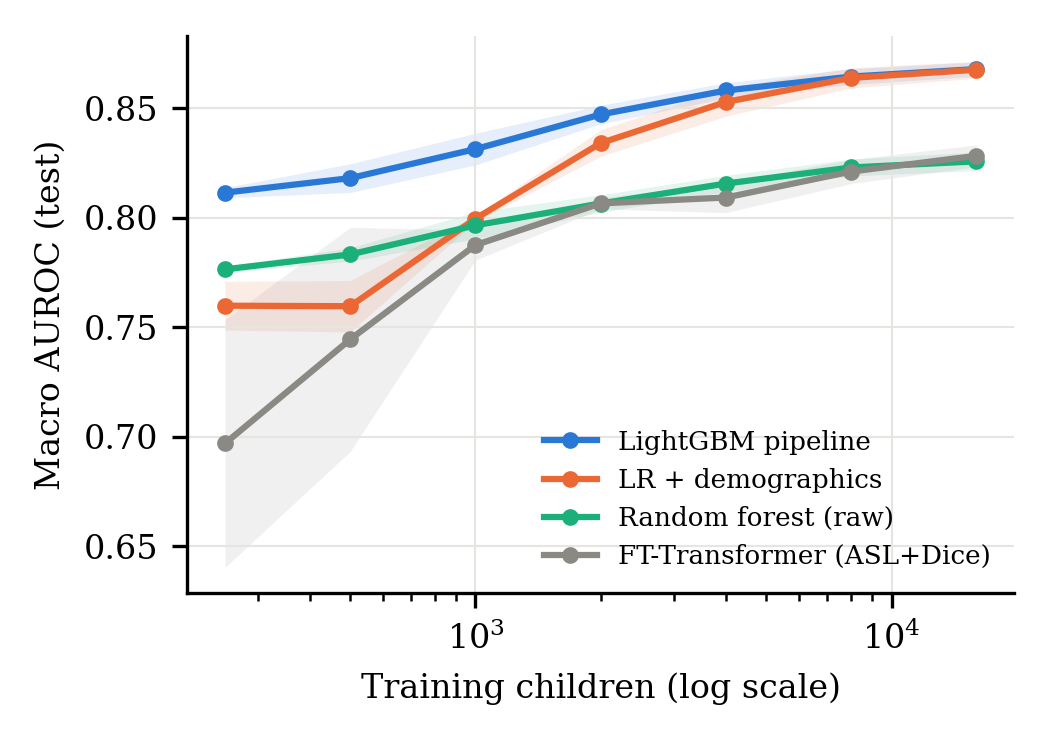
\includegraphics[width=\columnwidth]{fig_lgbm_learning_curve.png}
\caption{Macro AUROC versus training-set size (mean\,$\pm$\,SD over three seeds).}
\label{fig:lc}
\end{figure}

\subsection{Sensitivity to the generator's assumptions}
Because the generator was designed by us, a reader may suspect that it favours the
proposed pipeline. Fig.~\ref{fig:sens} varies each assumption. The pipeline is best,
or within 0.005 of the best model, in all 22 settings. It beats the ASL
FT-Transformer in 22 of 22 and the BCE FT-Transformer in 21 of 22, and the model
ranking stays stable (mean Kendall $\tau{=}0.89$ against the baseline ranking,
minimum 0.62).

One setting qualifies this. With no age effect (age slope 0), all models converge to
0.84--0.85 and the BCE FT-Transformer is marginally best (0.854 vs.\ 0.853). The
pipeline's advantage therefore comes mainly from handling the age and language
confounds through norming, not from the learning algorithm. It remains the right
choice because raw task scores do change with age, but the gain should be attributed
to norming.

\begin{figure*}[!t]
\centering
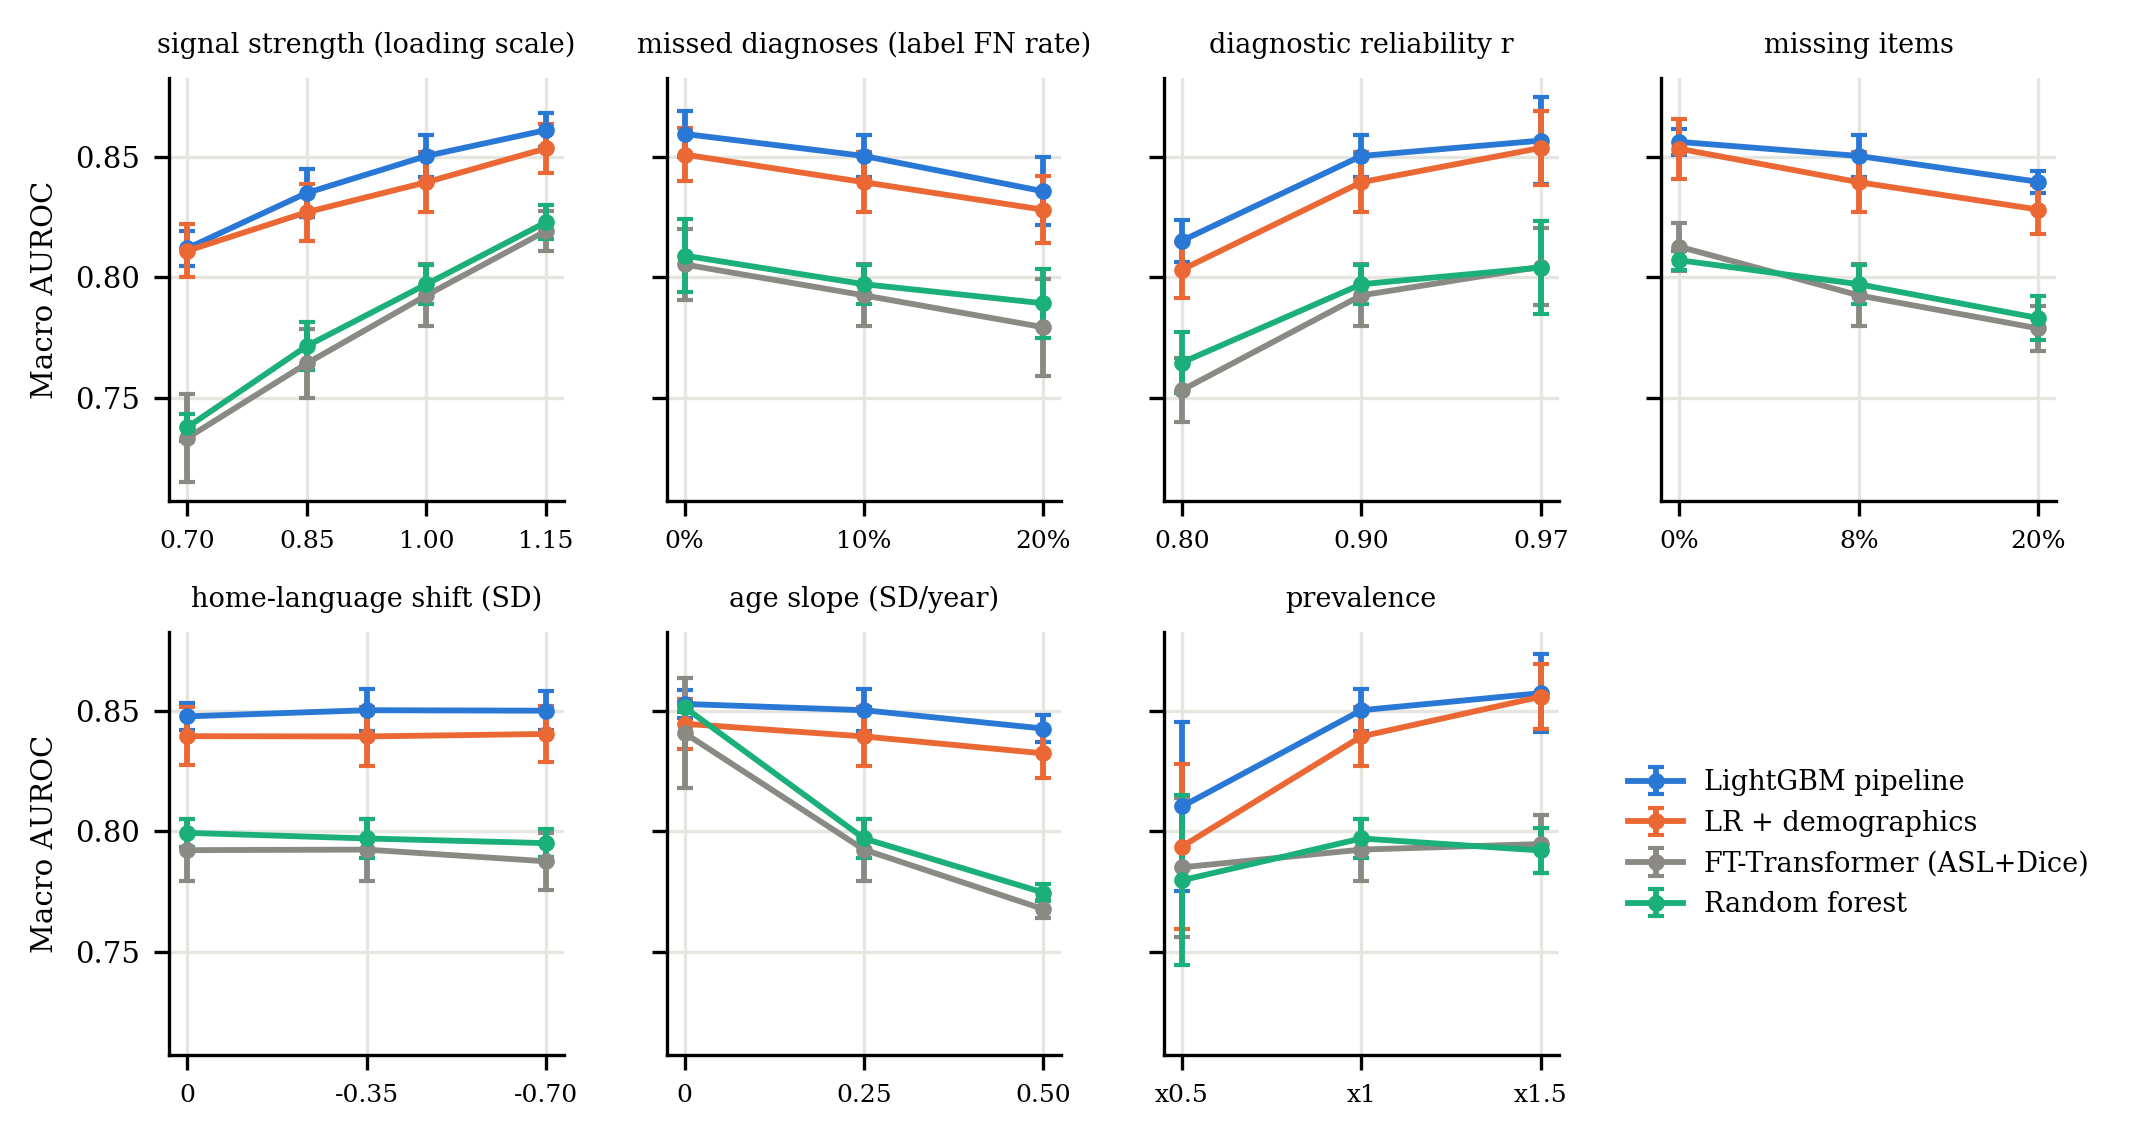
\includegraphics[width=0.92\textwidth]{fig_sensitivity.png}
\caption{Generator sensitivity analysis: macro AUROC (mean\,$\pm$\,SD, three seeds) as one assumption is varied at a time; the baseline setting is the middle value of each panel.}
\label{fig:sens}
\end{figure*}

\subsection{The screening operating point}
At sensitivity 0.86 the pipeline has specificity 0.685 and PPV 0.178 (95\% CI
0.168--0.188) at a prevalence of 6--8\%, and NPV 0.984. In a school of 500 children
this means about 180 referrals per disorder (34 true and 145 false positives) to
find 34 of the 40 affected children. The tool is therefore best used as a first, high-sensitivity stage that
rules children out and prioritises observation, not as a referral trigger on its own.

\subsection{Calibration and uncertainty}
The pipeline's probabilities are calibrated without post-processing (ECE 0.017). ASL
shifts probabilities upward (ECE 0.275) and temperature scaling makes this worse
(0.314), because one temperature rescales logits but cannot remove a bias
(Fig.~\ref{fig:calib}). The originally deployed conformal intervals, with hard-coded
widths, covered 0\% of test children; standard split-conformal sets covered 90\%
overall but only 52--64\% of affected children. The class-conditional sets cover
0.94 of affected and 0.90 of unaffected children. About a third to a half of
children receive the \emph{uncertain} set. This reflects the real limits of the data
and leads to a re-screen rather than a confident wrong answer.

\begin{figure}[!t]
\centering
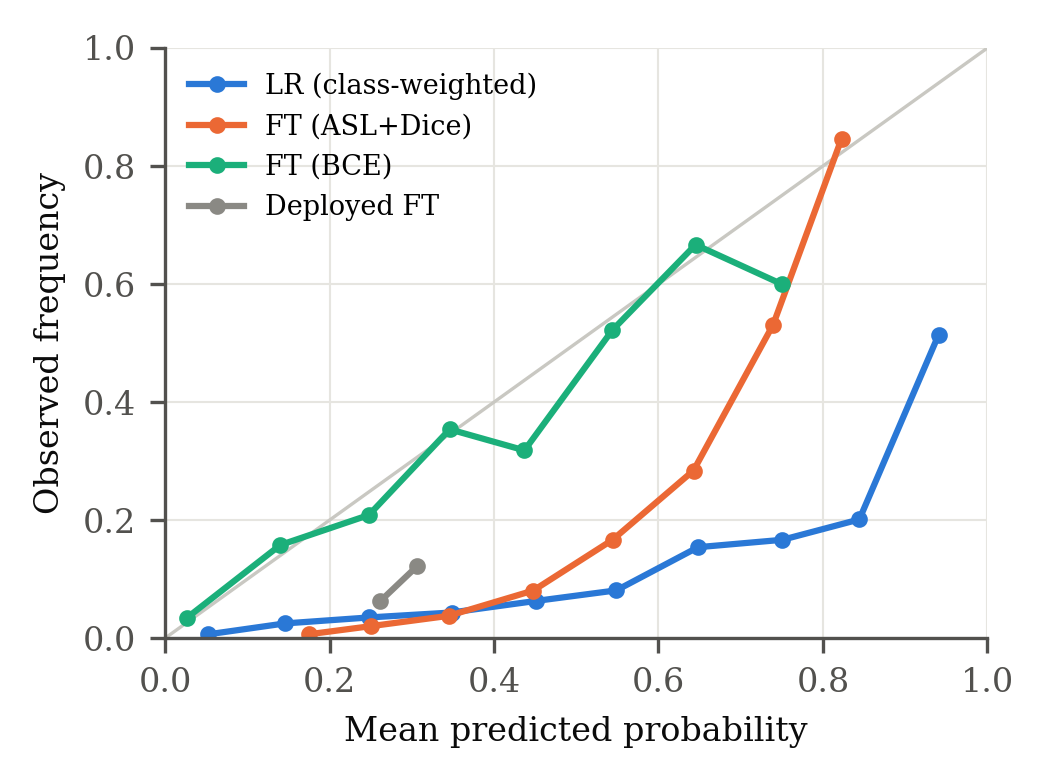
\includegraphics[width=\columnwidth]{fig_calibration.png}
\caption{Reliability diagram (seed 0, all disorders pooled). ASL-trained and class-weighted models overestimate risk; BCE lies close to the diagonal.}
\label{fig:calib}
\end{figure}

\subsection{Single tests, missing data and fairness}
Single-test models reach 0.848--0.855 AUROC, against 0.854--0.860 for the
comprehensive model, and clearly beat the original 0.5-fill path (0.741--0.781).
With up to 40\% additional items missing, the pipeline falls from 0.858 to 0.813,
degrading less than LR (to 0.757) and staying ahead of every model
(Fig.~\ref{fig:missing}).

Without covariates, Hindi-dominant children had higher dyslexia false-positive rates
(0.48 vs.\ 0.38 for the FT-Transformer) and 7--8-year-olds far higher ones than
11--12-year-olds (0.62 vs.\ 0.25), as shown in Fig.~\ref{fig:fair}. With norming, the
deployed bundle's false-positive rates by language are 0.33/0.38 (dyslexia),
0.35/0.34 (dyscalculia) and 0.28/0.30 (dysgraphia). The age gap is reduced but not
removed (e.g.\ 0.41 vs.\ 0.30 for dyslexia), partly because 15\% of training
covariates were masked to prepare for missing inputs.

\begin{figure}[!t]
\centering
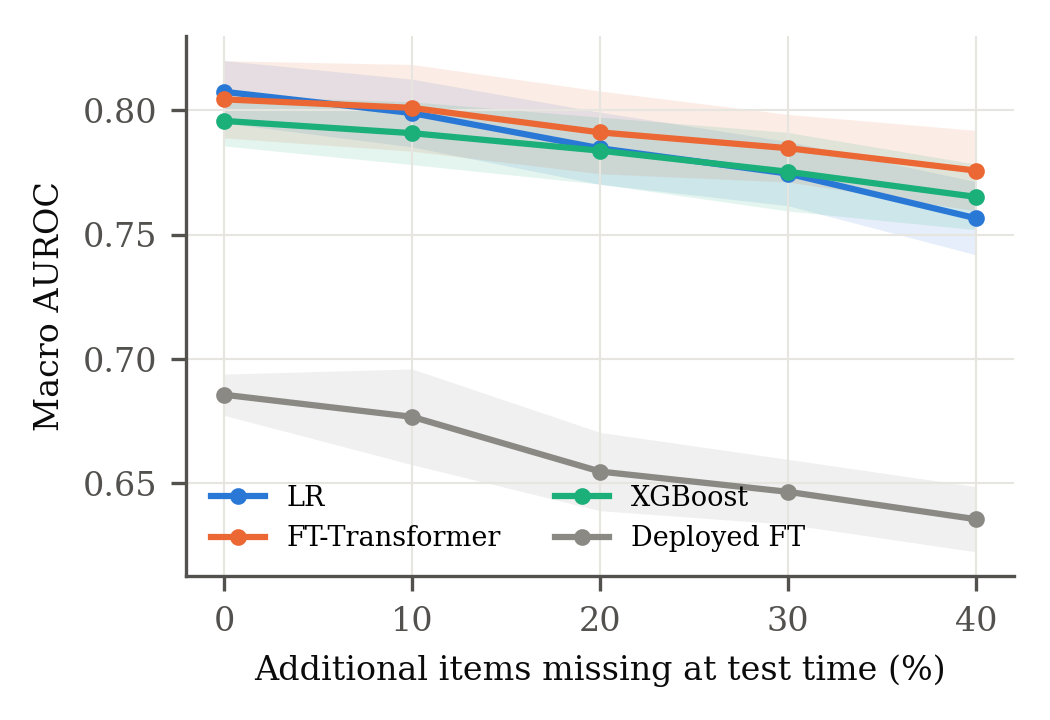
\includegraphics[width=\columnwidth]{fig_missing.png}
\caption{Macro AUROC as additional items are removed at test time (mean\,$\pm$\,SD over five seeds).}
\label{fig:missing}
\end{figure}

\begin{figure}[!t]
\centering
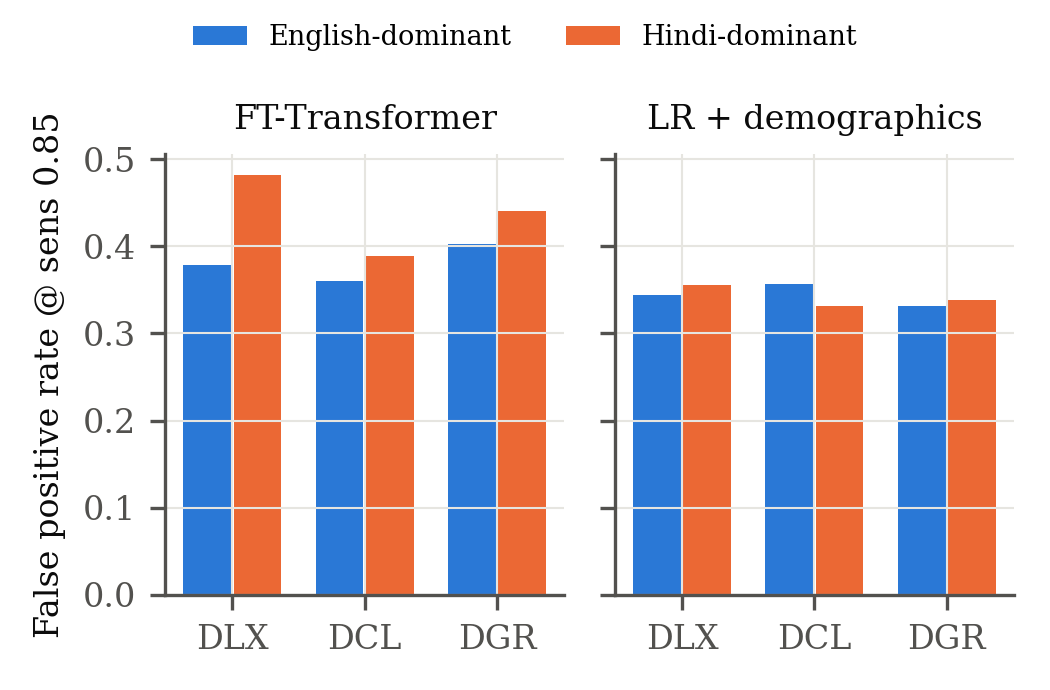
\includegraphics[width=\columnwidth]{fig_fairness.png}
\caption{False-positive rate by home language at the refer threshold, without (left) and with (right) demographic adjustment. DLX/DCL/DGR: dyslexia, dyscalculia, dysgraphia.}
\label{fig:fair}
\end{figure}

\subsection{Handwriting analysis}
Table~\ref{tab:hw} compares the original and new dysgraphia scorers on synthetic
handwriting. The original scorer gave neat writing 85--86 on a 60\,Hz pen but only
60--62 on a touch screen and 54--56 with a mouse, below the scores it gave writers
with tremor (78--82) or size and drift problems (81--84). It was measuring the
device. The new scorer gives all nine neat writers 99--100 and a low risk on every
device. It flags all nine tremor, stop-start and layout writers, and 2 of 3 distorted
writers, with the lowest domain matching the simulated deficit in each case.

Legibility from the self-hosted recogniser was 1.00 for neat writing on every device,
0.88 for size and drift problems, 0.79 for distorted and 0.70 for tremor writing.
Writing a different word than the prompt scores 0.

\begin{figure}[!t]
\centering
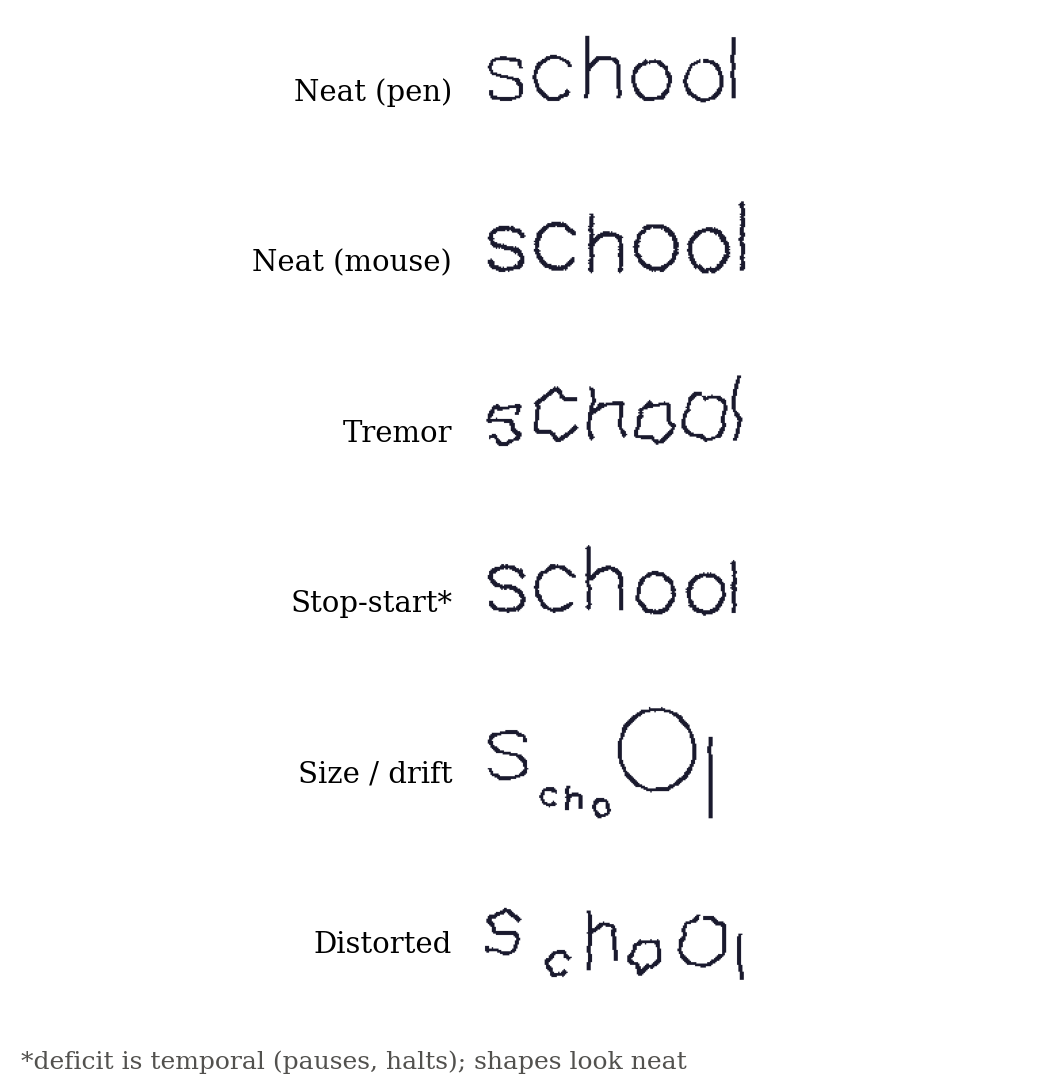
\includegraphics[width=0.92\columnwidth]{fig_handwriting_samples.png}
\caption{Synthetic handwriting of the word ``school'' for six of the seven profiles.}
\label{fig:hw}
\end{figure}

\begin{table}[!t]
\centering
\caption{Dysgraphia scores (0--100, three writers per profile) with the original and the new analysis; risk L/M/H = low/moderate/high.}
\label{tab:hw}
\footnotesize
\setlength{\tabcolsep}{3pt}
\begin{tabular}{@{}lccc@{}}
\toprule
Profile & Original & New (risk) & Legibility \\
\midrule
Neat, pen & 85--86 & 100 (L,L,L) & 1.00 \\
Neat, touch & 60--62 & 100 (L,L,L) & 1.00 \\
Neat, mouse & 54--56 & 99--100 (L,L,L) & 1.00 \\
Tremor & 78--82 & 72--78 (M,H,H) & 0.70 \\
Stop-start & 56--58 & 86--90 (M,M,M) & 1.00 \\
Size / drift & 81--84 & 75--86 (H,H,M) & 0.88 \\
Distorted & 69--72 & 75--88 (H,M,L) & 0.79 \\
\bottomrule
\end{tabular}
\end{table}

\subsection{Speech recognition and latency}
On 20 synthetic spoken sentences (two Windows voices, including number words) the
self-hosted Whisper model made no word errors, with a median latency of 0.44\,s per
clip on an RTX~2050 laptop GPU; speech and handwriting models together use 2.7\,GB of
GPU memory. These clips are clean adult speech, so this shows that the service works,
not how accurate it is for children or for Hindi.

\subsection{DSM-5 profile and Criterion D}\label{sec:dsm5res}
Adding the questionnaire to the tests does not improve discrimination
(Table~\ref{tab:dsm5}): macro AUROC 0.859 against 0.858 for tests alone, a paired
bootstrap difference of $+0.0014$ (95\% CI $-0.0016$ to $0.0045$). The teacher's view
is largely redundant with what the tests measure, and its halo and language bias add
noise. The questionnaire alone reaches only 0.743, so ratings cannot replace the tests.
The tests-plus-questionnaire model degrades gracefully without the questionnaire
(0.853). With or without the questionnaire, language learners who do not have a
disorder are flagged more often than fluent children (36\% vs.\ 30\%): norming
reduces this gap but does not close it, which is what Criterion~D is for.

Applying the Criterion~D rule (refer only children without a recorded D factor in the
flagged domain) cuts the refer rate from 35.5\% to 27.1\% and raises specificity from
0.684 to 0.760, but sensitivity falls from 0.860 to 0.681 and PPV barely moves (0.178
to 0.187): 21\% of true positives and 25\% of false positives are routed to review.
D factors are common in children with and without a disorder, so they cannot
separate the two. The rule should therefore defer, not exclude: such children are
re-screened after the factor is addressed (glasses, hearing check, language support).

\begin{table*}[!t]
\centering
\caption{DSM-5 profile evaluation, macro over three disorders and five seeds. FPR at the refer threshold among children without the disorder.}
\label{tab:dsm5}
\footnotesize
\setlength{\tabcolsep}{6pt}
\begin{tabular}{@{}lcccccc@{}}
\toprule
Model & AUROC & Ext. & Spec. & PPV & \multicolumn{2}{c}{FPR} \\
 & & & & & fluent & learner \\
\midrule
Tests + questionnaire & \pmsd{0.859}{.015} & 0.849 & 0.684 & 0.178 & 0.302 & 0.360 \\
Tests only & \pmsd{0.858}{.013} & 0.842 & 0.680 & 0.177 & 0.309 & 0.356 \\
\quad questionnaire withheld & \pmsd{0.853}{.012} & -- & 0.664 & 0.170 & 0.323 & 0.377 \\
Questionnaire only & \pmsd{0.743}{.030} & 0.738 & 0.395 & 0.102 & 0.593 & 0.644 \\
LR + covariates (tests) & \pmsd{0.849}{.014} & 0.835 & 0.647 & 0.164 & 0.341 & 0.392 \\
\midrule
\multicolumn{7}{@{}l}{Criterion D rule: sens.\ 0.860$\to$0.681, spec.\ 0.684$\to$0.760, refer rate 35.5\%$\to$27.1\%} \\
\bottomrule
\end{tabular}
\end{table*}

\subsection{Oral reading fluency under recognition errors}
With a clean transcript the alignment recovers WCPM within 0.3--2.5 words per minute
(Table~\ref{tab:orf}); the small upward bias comes from long misread words one letter
off, which the slip tolerance counts as correct. Recognition errors look like reading
errors, so WCPM is biased downwards roughly in proportion to the WER, while the
ranking of readers is preserved ($r\geq0.98$). At a fixed 25th-percentile cut-off the
flag keeps its sensitivity ($\geq$0.96) but its specificity falls from 0.96 at 5\% WER
to 0.89--0.95 at 10\% and 0.77--0.90 at 20\%. Counting transcript words without
alignment overestimates WCPM by 4--13 because misread and repeated words are counted.
Children's read speech, especially in Hindi, may well reach 10--20\% WER, so the
recogniser's error rate must be measured locally and either the cut-off shifted or
flagged readings confirmed by the teacher.

\begin{table}[!t]
\centering
\caption{WCPM recovered from simulated readers by recogniser WER (2000 readers per cell). Bias and MAE in words per minute; sensitivity and specificity of the below-25th-percentile flag.}
\label{tab:orf}
\footnotesize
\setlength{\tabcolsep}{3pt}
\begin{tabular}{@{}llrrccc@{}}
\toprule
Grade & WER & Bias & MAE & $r$ & Sens. & Spec. \\
\midrule
1 & 0\% & $+$0.2 & 0.3 & 0.999 & 0.99 & 1.00 \\
  & 10\% & $-$4.6 & 4.6 & 0.992 & 0.99 & 0.95 \\
  & 20\% & $-$9.5 & 9.5 & 0.982 & 0.99 & 0.90 \\
3 & 0\% & $+$1.7 & 1.8 & 0.999 & 0.96 & 1.00 \\
  & 5\% & $-$2.0 & 3.2 & 0.996 & 0.97 & 0.96 \\
  & 10\% & $-$6.2 & 6.5 & 0.995 & 1.00 & 0.92 \\
  & 20\% & $-$13.8 & 13.9 & 0.990 & 1.00 & 0.79 \\
5 & 0\% & $+$2.4 & 2.5 & 0.999 & 0.96 & 1.00 \\
  & 10\% & $-$7.6 & 8.1 & 0.995 & 1.00 & 0.89 \\
  & 20\% & $-$18.2 & 18.3 & 0.992 & 1.00 & 0.77 \\
\bottomrule
\end{tabular}
\end{table}

%=====================================================================
\section{Lessons from the Deployment Audit}\label{sec:audit}
%=====================================================================
Executable checks confirmed 17 defects in the originally deployed system
(Table~\ref{tab:defects}). Three of them combined to stop the screen working.
\begin{enumerate}
\item \emph{Train/serve skew}~\cite{sculley2015}: the network was trained on
standardised features but served raw $[0,1]$ values.
\item \emph{Artefact mismatch}: the served checkpoint stored no thresholds, so the
engine used \texttt{thresholds.json} and \texttt{temperature.json} from an earlier run.
\item \emph{Regime mismatch}: thresholds fitted on deterministic probabilities were
applied to Monte-Carlo-dropout averages of tempered probabilities.
\end{enumerate}
Served scores lay between 0.22 and 0.33 while the thresholds were 0.91--0.93, so the
screen flagged no child (sensitivity 0). Through the public API, a severely impaired
simulated reader scored 0.264 and a strong reader 0.247, both ``Low''. Legacy
per-disorder ``neural'' predictors used untrained random weights (AUROC 0.475).

The lessons we draw are general.
(i)~Ship model, preprocessing and thresholds as one verified artefact.
(ii)~Test behaviour end to end, for example that risk rises with impairment through
the API, not only status codes.
(iii)~Compare models at the same pre-registered operating point; at a fixed 0.5
threshold, ASL's upward shift looked like extra sensitivity.
(iv)~Compute uncertainty and fairness claims from model outputs, never hard-code them.
(v)~Check that each measure tracks the child, not the device.
The fixes are in place and covered by regression tests, including a test that every
risk tier is reachable and that neat handwriting scores highly on all devices.

\begin{table}[!t]
\centering
\caption{Main defects found in the original deployment (C = critical, H = high, M = medium).}
\label{tab:defects}
\footnotesize
\setlength{\tabcolsep}{3pt}
\begin{tabular}{@{}lp{7.0cm}@{}}
\toprule
Sev. & Defect \\
\midrule
C & Serving omitted the training-time feature standardisation \\
C & Checkpoint, thresholds and temperature came from different runs \\
C & Impaired and strong readers both scored ``Low'' end to end \\
H & Thresholds 0.91--0.93; ``High'' tier unreachable ($1.1t>1$) \\
H & Early stopping restored the last epoch (live \texttt{state\_dict} reference) \\
H & Temperature scaling shipped although it raised ECE from 0.274 to 0.316 \\
H & ``90\% guaranteed'' conformal widths hard-coded (0\% coverage) \\
H & Fairness status hard-coded; audit scored fabricated predictions \\
H & Legacy predictors with untrained random weights \\
H & Benchmark generator effect size $d\approx1.5$ (stated 0.6) \\
H & Handwriting scores driven by device sampling rate; no legibility check \\
M & Warm-up stepped per epoch but counted in batches (130 epochs) \\
M & Benchmark compared models at a fixed 0.5 threshold \\
\bottomrule
\end{tabular}
\end{table}

%=====================================================================
\section{Discussion}
%=====================================================================
On data that reflects real measurement conditions, the transformer, asymmetric loss
and label-correlation layer add complexity without improving accuracy. What helps is
measuring the child correctly: norming for age and language, handling missing inputs
explicitly, calibrating before thresholding, giving uncertainty guarantees to the
affected class, and making handwriting measures independent of the device. These
changes also make the system easier to audit. The LightGBM bundle is a small file
whose preprocessing, thresholds and checksums are verified at load.

Three practical points follow. First, the frontend must collect age and home language;
without them, AUROC falls by 0.055 and specificity on the external site halves.
Second, a single-stage screen at sensitivity 0.85 refers many children (PPV 0.18), so
it should be a first stage. Third, the largest remaining uncertainty is the synthetic
data itself, which only real labelled data can resolve. The system now stores every
assessment with its model version and accepts confirmed diagnoses for that purpose.

DSM-5 alignment changes what the screen says more than how well it ranks children.
The questionnaire did not raise AUROC, and we do not claim it does; its role is to
record what tests cannot observe (persistence despite help, onset, and other
explanations) and to stop the screen from treating a child who is learning the
language of instruction, or who needs glasses, as a likely case of dyslexia. Because
Criterion~D factors are common among true cases as well, the right action for them is
``address and re-screen'', not exclusion.

\section{Limitations}\label{sec:limits}
All results are synthetic. The latent structure, loadings, confound sizes and noise
levels are literature-informed choices, not estimates from SwarSetu data. The
sensitivity analysis shows that the model ranking is robust to these choices within
the ranges tested, but real data may contain effects we did not model (practice,
motivation, examiner and dialect effects). The handwriting thresholds were set on
synthetic writing and need norms from real children by grade and device. The
handwriting recogniser was trained on adult English handwriting and does not read
Devanagari. The speech check used clean adult synthetic speech. The DSM-5
questionnaire has not been validated (reliability, agreement with specialists), its
teacher ratings were simulated with assumed accuracy and bias, and the written
expression scores depend on teacher judgement. Reading-fluency norms are US English
norms~\cite{hasbrouck2017}; there are no Hindi norms, and the fact-fluency benchmarks
are approximate. Absolute numbers
should not be quoted as clinical accuracy. A prospective study with blinded
specialist assessment is required before clinical use, with ethics approval and
parental consent.

\section{Conclusion}
We replaced an over-easy benchmark with a realistic synthetic one and used it to
build and stress-test a screen for dyslexia, dyscalculia and dysgraphia. A LightGBM
pipeline on age- and language-normed features beat every alternative, including the
originally proposed FT-Transformer, with statistically clear margins. It was
calibrated, gave class-conditional coverage guarantees and narrowed subgroup gaps, and
its advantage held across 22 variations of the generator. A device-invariant
handwriting analysis with self-hosted legibility recognition corrected a scorer that
had penalised neat writing on touch screens. Speech recognition now runs on a
self-hosted model. A stored student profile and teacher questionnaire now cover DSM-5
Criteria A, C and D, and each test reports the DSM-5 specifiers. The questionnaire
does not improve discrimination, but it makes referrals interpretable and identifies
children whose difficulties have another explanation. The audit shows that, for such
systems, measurement and pipeline integrity matter more than model architecture.

\section*{Data and Code Availability}
Cohort generator: \texttt{backend/screening/synthetic\_cohort.py}; pipeline:
\texttt{backend/screening/}; evaluations: \texttt{backend/reports/realistic\_eval/}
(\texttt{evaluate\_all\_models.py}, \texttt{lightgbm\_dynamics.py},
\texttt{sensitivity\_bootstrap.py}, \texttt{dsm5\_evaluation.py},
\texttt{defect\_checks.py}); DSM-5 questionnaire and criteria logic:
\texttt{backend/screening/dsm5.py}; reading-fluency simulation:
\texttt{frontend/src/test/orfSimulation.test.ts}; handwriting analysis:
\texttt{frontend/src/lib/dysgraphiaAnalysis.ts} with synthetic handwriting fixtures
and regression tests in \texttt{frontend/src/test/}.

\section*{Acknowledgment}
[Funding and acknowledgements.] Following IEEE policy, we disclose that an AI
assistant was used to help write code, run analyses and draft and edit the text; the
authors reviewed all content and are responsible for it.

\begin{thebibliography}{99}
\bibitem{dsm5} American Psychiatric Association, \emph{Diagnostic and Statistical Manual of Mental Disorders}, 5th ed. Arlington, VA: APA, 2013.
\bibitem{willcutt2013} E.~G. Willcutt \emph{et al.}, ``Comorbidity between reading disability and math disability: Concurrent psychopathology, functional impairment, and neuropsychological functioning,'' \emph{J. Learn. Disabil.}, vol.~46, no.~6, pp.~500--516, 2013.
\bibitem{landerl2010} K.~Landerl and K.~Moll, ``Comorbidity of learning disorders: Prevalence and familial transmission,'' \emph{J. Child Psychol. Psychiatry}, vol.~51, no.~3, pp.~287--294, 2010.
\bibitem{pennington2006} B.~F. Pennington, ``From single to multiple deficit models of developmental disorders,'' \emph{Cognition}, vol.~101, no.~2, pp.~385--413, 2006.
\bibitem{rello2015} L.~Rello and M.~Ballesteros, ``Detecting readers with dyslexia using machine learning with eye tracking measures,'' in \emph{Proc. W4A}, 2015, pp.~1--8.
\bibitem{asselborn2018} T.~Asselborn \emph{et al.}, ``Automated human-level diagnosis of dysgraphia using a consumer tablet,'' \emph{npj Digit. Med.}, vol.~1, art.~42, 2018.
\bibitem{benbaruch2021} E.~Ben-Baruch \emph{et al.}, ``Asymmetric loss for multi-label classification,'' in \emph{Proc. IEEE/CVF ICCV}, 2021, pp.~82--91.
\bibitem{gal2016} Y.~Gal and Z.~Ghahramani, ``Dropout as a Bayesian approximation: Representing model uncertainty in deep learning,'' in \emph{Proc. ICML}, 2016, pp.~1050--1059.
\bibitem{guo2017} C.~Guo, G.~Pleiss, Y.~Sun, and K.~Q. Weinberger, ``On calibration of modern neural networks,'' in \emph{Proc. ICML}, 2017, pp.~1321--1330.
\bibitem{youden1950} W.~J. Youden, ``Index for rating diagnostic tests,'' \emph{Cancer}, vol.~3, no.~1, pp.~32--35, 1950.
\bibitem{lundberg2020} S.~M. Lundberg \emph{et al.}, ``From local explanations to global understanding with explainable AI for trees,'' \emph{Nat. Mach. Intell.}, vol.~2, pp.~56--67, 2020.
\bibitem{falconer1965} D.~S. Falconer, ``The inheritance of liability to certain diseases, estimated from the incidence among relatives,'' \emph{Ann. Hum. Genet.}, vol.~29, no.~1, pp.~51--76, 1965.
\bibitem{melbylervag2012} M.~Melby-Lerv{\aa}g, S.-A.~H. Lyster, and C.~Hulme, ``Phonological skills and their role in learning to read: A meta-analytic review,'' \emph{Psychol. Bull.}, vol.~138, no.~2, pp.~322--352, 2012.
\bibitem{breiman2001} L.~Breiman, ``Random forests,'' \emph{Mach. Learn.}, vol.~45, no.~1, pp.~5--32, 2001.
\bibitem{chen2016} T.~Chen and C.~Guestrin, ``XGBoost: A scalable tree boosting system,'' in \emph{Proc. ACM SIGKDD}, 2016, pp.~785--794.
\bibitem{ke2017} G.~Ke \emph{et al.}, ``LightGBM: A highly efficient gradient boosting decision tree,'' in \emph{Proc. NeurIPS}, 2017, pp.~3146--3154.
\bibitem{collins2015} G.~S. Collins, J.~B. Reitsma, D.~G. Altman, and K.~G.~M. Moons, ``Transparent reporting of a multivariable prediction model for individual prognosis or diagnosis (TRIPOD): The TRIPOD statement,'' \emph{BMJ}, vol.~350, g7594, 2015.
\bibitem{grinsztajn2022} L.~Grinsztajn, E.~Oyallon, and G.~Varoquaux, ``Why do tree-based models still outperform deep learning on typical tabular data?'' in \emph{Proc. NeurIPS Datasets and Benchmarks}, 2022.
\bibitem{angelopoulos2021} A.~N. Angelopoulos and S.~Bates, ``A gentle introduction to conformal prediction and distribution-free uncertainty quantification,'' arXiv:2107.07511, 2021.
\bibitem{vovk2005} V.~Vovk, A.~Gammerman, and G.~Shafer, \emph{Algorithmic Learning in a Random World}. New York: Springer, 2005.
\bibitem{hardt2016} M.~Hardt, E.~Price, and N.~Srebro, ``Equality of opportunity in supervised learning,'' in \emph{Proc. NeurIPS}, 2016, pp.~3315--3323.
\bibitem{gorishniy2021} Y.~Gorishniy, I.~Rubachev, V.~Khrulkov, and A.~Babenko, ``Revisiting deep learning models for tabular data,'' in \emph{Proc. NeurIPS}, 2021, pp.~18932--18943.
\bibitem{sculley2015} D.~Sculley \emph{et al.}, ``Hidden technical debt in machine learning systems,'' in \emph{Proc. NeurIPS}, 2015, pp.~2503--2511.
\bibitem{efron1993} B.~Efron and R.~J. Tibshirani, \emph{An Introduction to the Bootstrap}. New York: Chapman \& Hall, 1993.
\bibitem{li2023trocr} M.~Li \emph{et al.}, ``TrOCR: Transformer-based optical character recognition with pre-trained models,'' in \emph{Proc. AAAI}, 2023, pp.~13094--13102.
\bibitem{radford2023whisper} A.~Radford \emph{et al.}, ``Robust speech recognition via large-scale weak supervision,'' in \emph{Proc. ICML}, 2023, pp.~28492--28518.
\bibitem{lacquaniti1983} F.~Lacquaniti, C.~Terzuolo, and P.~Viviani, ``The law relating the kinematic and figural aspects of drawing movements,'' \emph{Acta Psychol.}, vol.~54, pp.~115--130, 1983.
\bibitem{hasbrouck2017} J.~Hasbrouck and G.~Tindal, ``An update to compiled ORF norms,'' Behavioral Research and Teaching, Univ. of Oregon, Eugene, OR, Tech. Rep. 1702, 2017.
\end{thebibliography}

\end{document}
